\documentclass[12pt]{article}
\usepackage{graphicx}
\begin{document}
\title{Lista 2 - Piramide Usando OpenGL - SDL2}
\author{Mac\'artur de Sousa Carvalho}
\maketitle

\section{Solu\c{c}\~ao Proposta}
	A solu\c{c}\~ao proposta nesta lista tr\^es \'e aprender a utilizar renderiza\c{c}\~ao de malhas triangulares
	em um programa utilizando SDL2 e OPENGL , se a utiliza\c{c}\~ao de um shader.O arquivo a ser lido como amostra 
	\'e um coelho no formato .off.Este formato \'e simples de ser lido e utilizado em programa feito na m\~ao.	
	
\section{Estrutura de Dados Proposta}
	As estruturas de dados utilizadas para fazer est\'a solu\c{c}\~ao foram: 
	  
	  - Mesh(Abstra\c{c}\~ao de malha triangular);
	  
	    Contendo os atributos:  
	      Xmin,Ymin,Zmin,Xmax,Ymax,Zmax,vetor de pontos,vetor de faces,inteiro indicando se tem textura,
	      inteiro indicando se tem cor, deltaX,deltaY,deltaZ, e um nFaces e nDots indicando a quantidade de pontos
	      a serem armazenados no Mesh.
	   
	  - Dot(Abstra\c{c}\~ao de pontos):
	    
	    Contendo os atributos:
	      x,y,z que armazena as cordendas dos pontos;
	      red,green,blue para armazenar os valores das cores nos pontos;
	      alpha para armazenar o valor do ponto \'e opaco ou transparente;
	      
	   - Face(Abstra\c{c}\~ao de faces do objeto):
	    
	     Contendo os atributos:
	     vetor de indices que armazena os 3 ou quatro indices 
	     passados na leitura do arquivo;
	
	
	
\section{A malha Poligonal}
    A malha poligonal \'e uma cole\c{c}\~ao de faces (onde cada face \'e um conjunto de v\'ertices)que
    definem um objeto tridimensional nos campos da computa\c{c}\~ao gr\'afica e da modelagem tridimensional.
    As faces geramente s\~ao constituidas de tri\^angulos (tamb\'em chamada de malha triangular )  ou quadril\'ateros, uma vez estas formas simplificam o processo de renderiza\c{c}\~ao 
    , no entanto tamb\'em tamb\'em podem ser compostas por formas geom\'etricas mais complexas.
  
\section{Principais formatos de arquivos de malhas 3D}
  Para a cria\c{c}\~ao de arquivos de formatos de arquivos de malha 3d existem farias extensões possiveis tais como:
  3DS(3D Studio) ,BLEN( BLENDER ), DAE (COLLADA) , DXF (AutoCAD) ,FBX ( Autodesk exchange), 
  LOW (Lightwave),OBJ,OFF,PLY,PTS,PTX,SC1(Sculptris),SCL(Pro/engineer),SKP(Google sketchup)
  ,STL,TRI,V3D,WRL (VRML) , X3D, X3DV, XSI(SoftImage), ZTL(Zbrush),XYZ.
  
  Todos eles possuem um maneira diferente de ser lido, para esta lista ser\'a citado a leitura do STL e do OBJ.
 
 \section*{STL}   
   O inicio da linha contem:  solid name, onde name é opcional. 
   
   O arquivo continua com a leitura de triangulos iniciando,com facet normal indicando o vetor normal,com valores ni,nj,nk,
   em seguida faz a leitura de todos os vertex do vetor.
   
   Por fim fecha-se o loop de captura do vetor,o facet e o solid.  
  
  Exemplo:
  
  
  Com name:
  
  solid name
  
  facet normal ni nj nk
  
  
        outer loop

        vertex v1x v1y v1z
 
        vertex v2x v2y v2z
 
        vertex v3x v3y v3z
      
      endloop
    
    endfacet
  
  endsolid name
  
  Sem name:
  
  solid 
  
    facet normal ni nj nk
    
      outer loop
      
       vertex v1x v1y v1z

       vertex v2x v2y v2z
 
       vertex v3x v3y v3z
  
       endloop
      
    endfacet
  
  endsolid 
 
 
 \section*{OBJ}
       Neste arquivo linhas iniciadas com '\#' s\~ao coment\'arios.
       
      Primeiramente \'e feito a leitura dos vertex, com 4 parametros, 
      onde o quarto \'e opcional e definido com default em 1.0.

      Exemplo de linha:
	v 0.123 0.234 0.345 1.0
	

      O outro valor lido a coordenadas das texturas , que recebem 3 parametros entre
      0 e 1 e o ultimo parametro \'e opcional e por default vale 0;
      
      Exemplo de linha:
       vt 0.5000 1 0
      
      Em segui \'e feito a leitura de vetores normais, tendo como magnitude unitaria
      
      Exemplo de linha:
      vn 0.707 0.000 0.707
      
      Em seguida \'e capturado parametros de espa\c{c}os do vertex.
      
      Exemplo de linha:
	vp 0.310000 3.210000 2.100000
	
      E por fim contem os valores das faces definidos como:
      
      f v1/ vt1 / vn1 ,
      
      a utiliza\c{c}\~ao de textura \'e opcional podendo ser retirada ficando
      
      f  v1 // vn1
      
      
      Exemplo de Arquivo:
      
      
      \# List of Vertices, with (x,y,z[,w]) coordinates, w is optional and defaults to 1.0.
  
      v 0.123 0.234 0.345 1.0
  
      v ...
  
     ...
  
     \# Texture coordinates, in (u ,v [,w]) coordinates, these will vary between 0 and 1, w is optional and default to 0.
  
     vt 0.500 1 [0]
  
     vt ...
  
     ...
  
     \# Normals in (x,y,z) form; normals might not be unit.
 
 
     vn 0.707 0.000 0.707
 
     vn ...
  
     ...

     \# Parameter space vertices in ( u [,v] [,w] ) form; free form geometry statement ( see below )

     vp 0.310000 3.210000 2.100000

     vp ...

     ...
 
    \# Face Definitions (see below)
  
     f 1 2 3
  
     f 3/1 4/2 5/3
 
     f 6/4/1 3/5/3 7/6/5
  
     f ...
  
     ...


   
\section{Principais Li\c{c}\~oes Aprendidas}
     Nesta lista foi possivel entender melhor o funcionamento de uma malha triangular utilizando opengl, e como realizar a leitura de
      de arquivos que utilizam formatos que armazenam malhas 3d.
\section{Principais Dificuldades Encontradas}
    As principais dificuldades encontradas foram ler todos os pontos de maneira que todos sejam armazenados de forma correta nas estruturas
    e a fun\c{c}\~ao que mais foi dificil de ser utilizada foi a de redimensionar , pois deve-se entender bem a teoria para se aplicar os calculos
    nas imagens.Sabendo todos as fun\c{c}ões que pode-se implementar fica bem facil de se realizar a renderiza\c{c}\~ao dos arquivos.

\section{Imagem solu\c{c}\~ao proposta}

\begin{figure}[!htb]
\centering
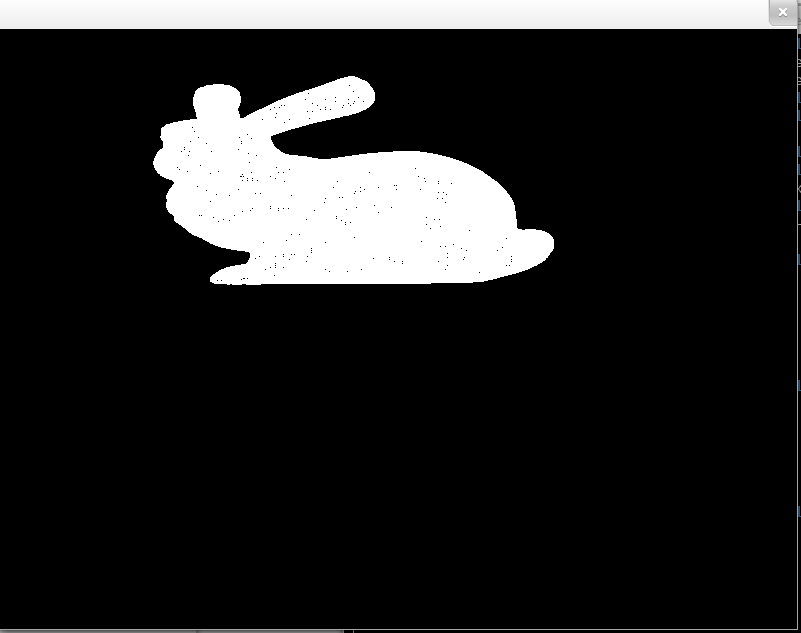
\includegraphics[scale=0.5]{images/rabit_line.png}
\caption{Figura utilizando Linhas(Vertices) de um coelho}
\end{figure}

\begin{figure}[!htb]
\centering
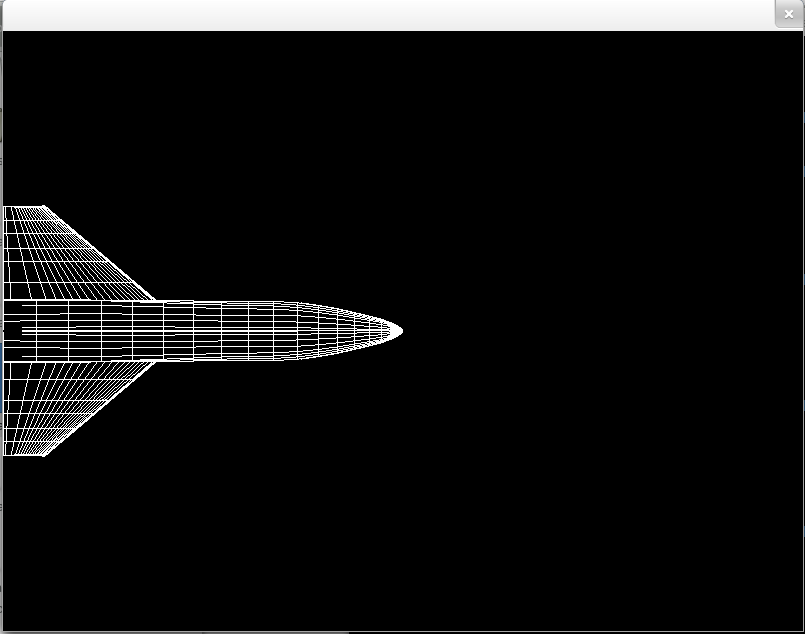
\includegraphics[scale=0.5]{images/space_shuttle_line.png}
\caption{Figura utilizando linhas para formar uma nave espacial}
\end{figure}

\begin{figure}[!htb]
\centering
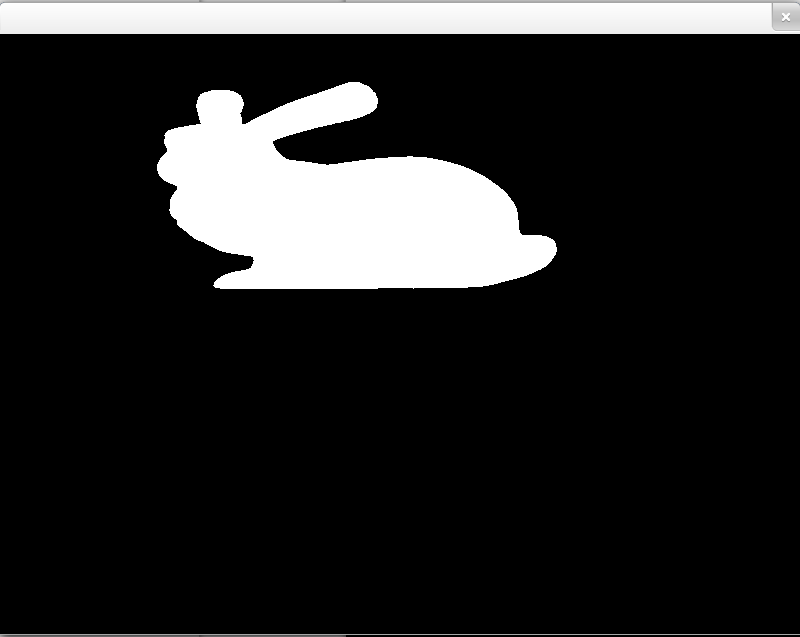
\includegraphics[scale=0.5]{images/rabit_polygon.png}
\caption{Figura utilizando poligonos para formar uma coelho}
\end{figure}


\end{document}
